\documentclass[paper=a4, fontsize=11pt]{article}
\usepackage[utf8]{inputenc}
\usepackage[english,magyar]{babel}
\usepackage{amsmath}
\usepackage{graphicx} 
\usepackage{float}
\usepackage{rotating}
\usepackage{latexsym}
\usepackage{blindtext}
\addtolength{\oddsidemargin}{-.875in}
\addtolength{\evensidemargin}{-.875in}
\addtolength{\textwidth}{1.95in}
\addtolength{\topmargin}{-.9in}
\addtolength{\textheight}{1.6in}



\title{\scshape\Huge Molekula Dinamika }
\date{\scshape\Large 2018.04.15.}
\author{\scshape\huge Nagy Péter\\\scshape\huge m07ilf}





\begin{document}

\maketitle
\newpage
\vspace{11cm}
\tableofcontents
\newpage
\section{Bevezetés}
A kisérlet célja számítógépes szimulációs környezetben megvalósított molekulák dinamikai vizsgálata. 

\section{Elméleti áttekintés}
A molekula dinamikai szimulációkban a részecskék jellemző darabszáma Avogadro szám nagyságrendű.Számítógéppel ennyi részecskét nem vagyunk képesek szimulálni, de képesek vagyunk annyi darabot, hogy arra már értelmezhető legyen a termodinamika törvényei. Folyamatos közelítéseket alkalmazva tudjuk növelni a szimulált részecskék darab számát, de ovatosnak kell leni nehogy tul durva közelítésekkel éljünk és teljesen eltávolodjunk a fizikai valóságtól. Legyen N darab olyan részecskénk a kisérletben amelyeknek tudjuk a kezdő pozicióját és a sebességét. A Newton törvények alapján számoljuk ki páronként a kölcsönhatásokat majd léptessük a rendszert.A rendszer egyensúlyi állapotában teljesül az enrgia ekvipartició tétel.
\begin{align}
< K >=< \frac{1}{2}mv^2 >=<\frac{3}{2}kT>
\end{align}
A szimuláció során <K> mutatja, hogy a rendszer egyensúlyban van-e. Egyensúlyban mérhetők a termodinamikai mennyiségek.

\section{Mérési feladatok}
\subsection{1.Feladat}
A feladat az md.cpp és az md2.cpp programok megértése és összehasonlítása volt. Az md.cpp egy Lennard-Jones szimuláció amely a velocity-Verlet algoritmussal léptet. A különbség az md2.cpp programban ott van, hogy a kezdeti sebességet Maxwell-Boltzmann eloszlás szerint generálja, figyeli a pillanatnyi hőmérsékletet és ha az nem felel meg a megjelölt értéknek akkor újra skáláza azt. Megfigyelhető, hogy az md2.cpp kimenetéből kapott eredmény esetében gyorsabban relaxál az egyensúlyi állapotába. De a kezdetben nagyobb ugrásokat produkál az újra skálázgatás miatt.
\begin{figure}[H]
    \centering
    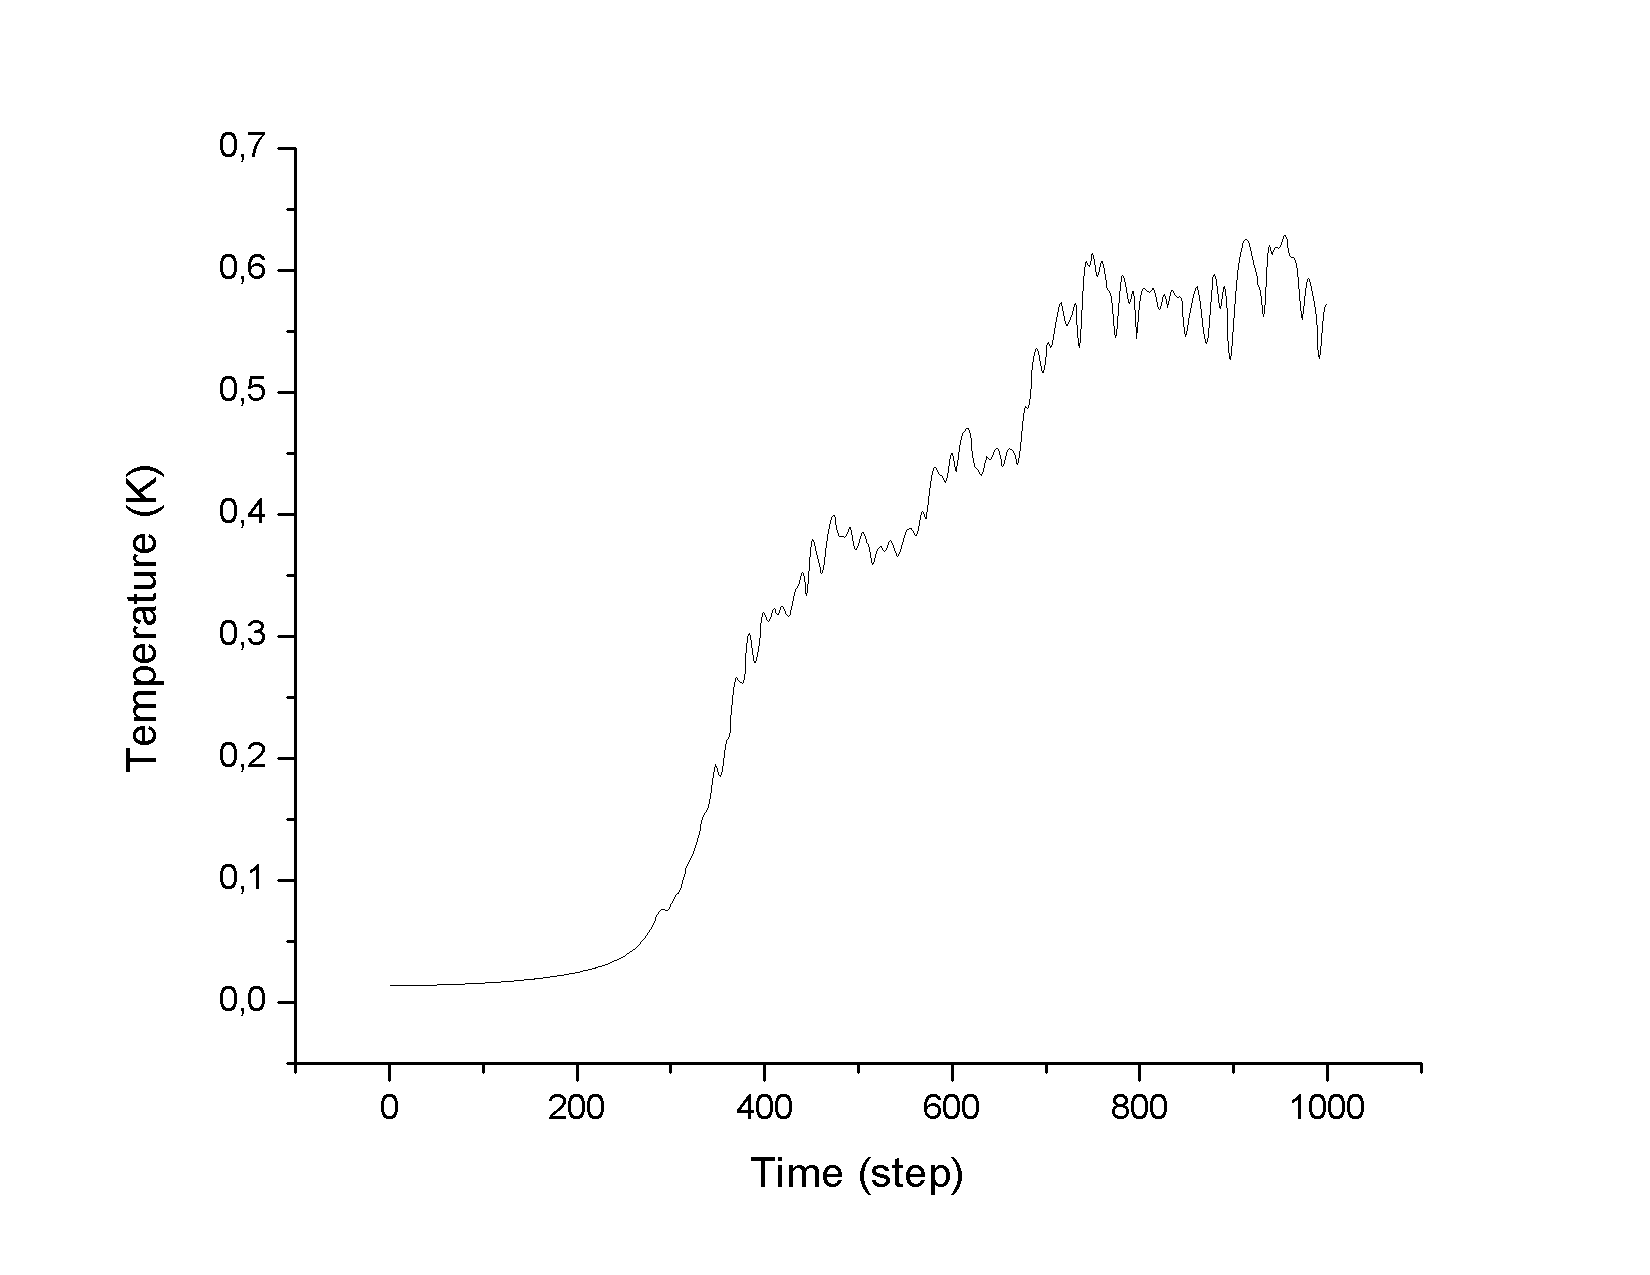
\includegraphics[width=0.75\textwidth]{md1}
    \caption{md1.cpp kimenete }
\end{figure}


\begin{figure}[H]
    \centering
    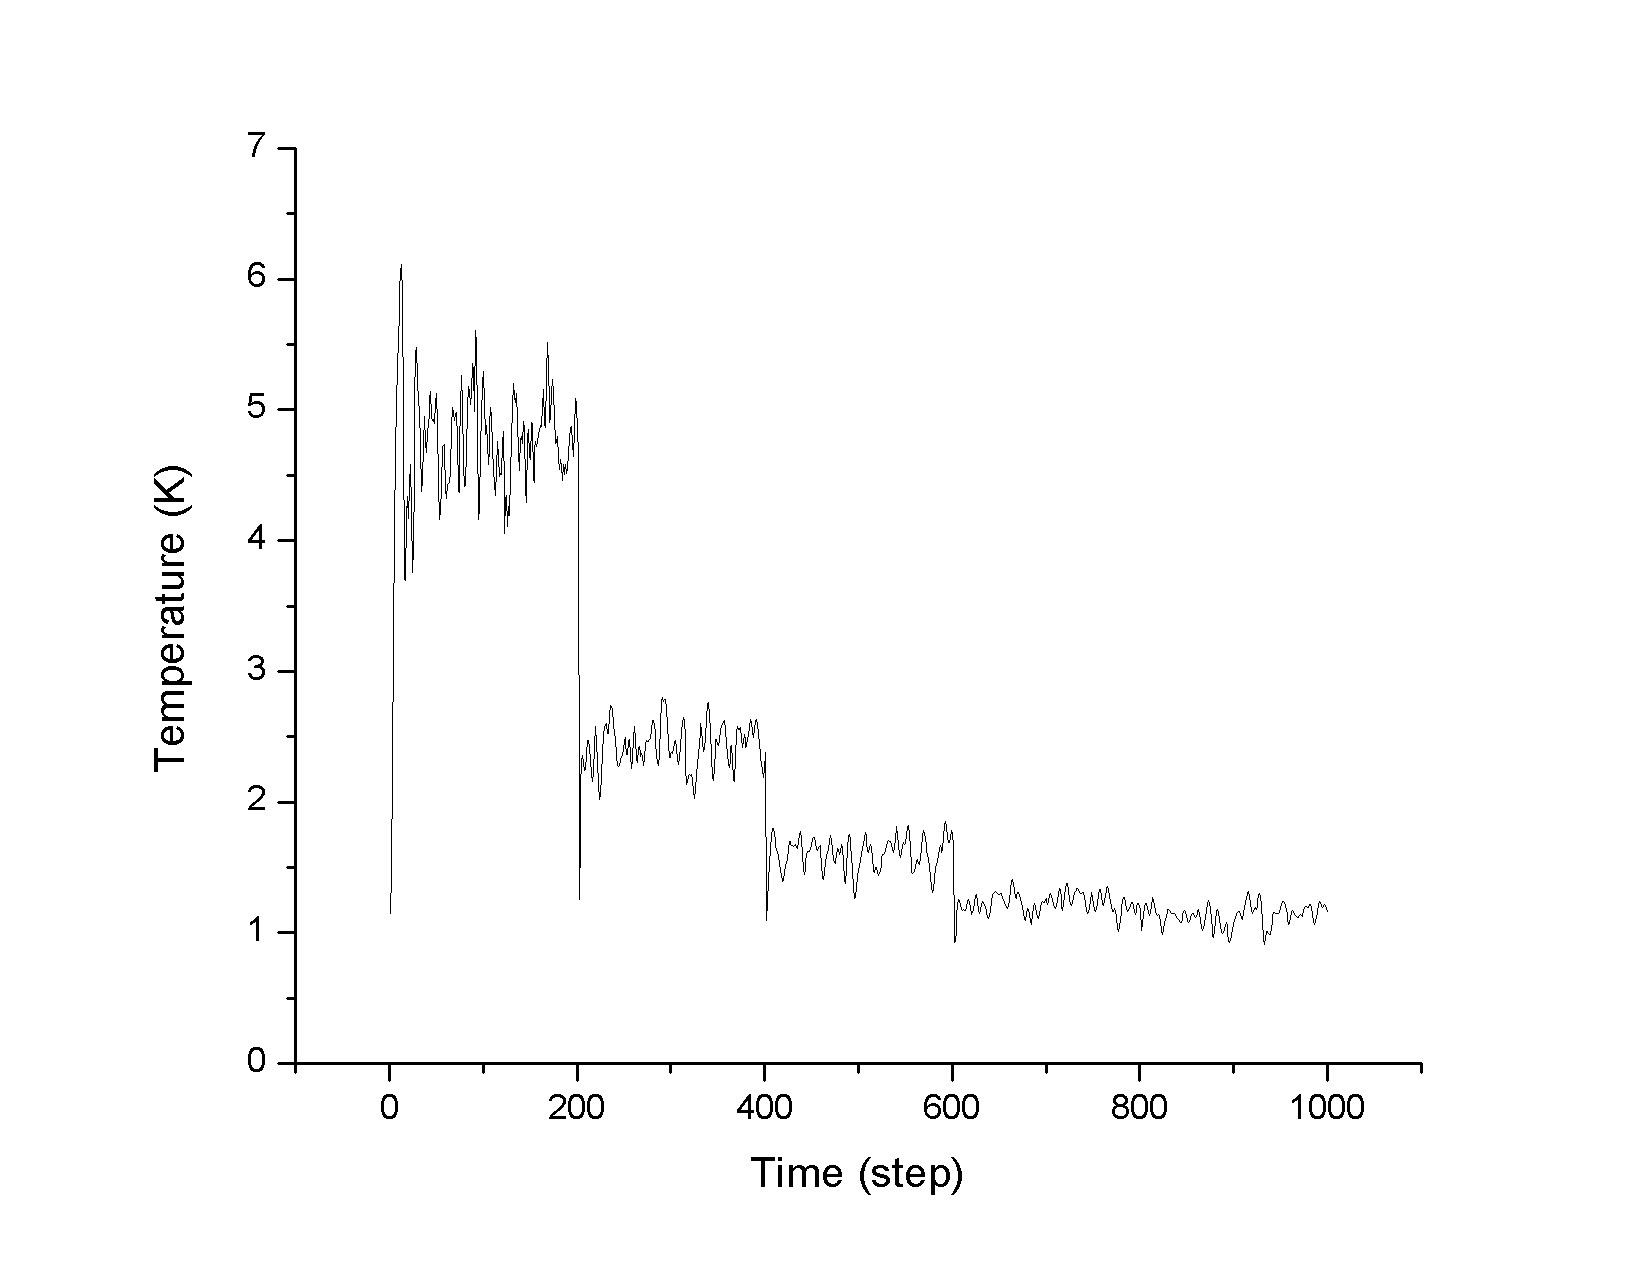
\includegraphics[width=0.75\textwidth]{md2}
    \caption{md1.cpp kimenete }
\end{figure}


\subsection{2.Feladat }
Az md3.cpp különböző egyszerűsítésekket használ, hogy javítsan az eredményt. Egy adott $r_{cutoff}$ érték felett 0 értéket ad a potenciálnakettől gyorsabb lesz az algoritmus. Az $r_{max}$ beállítja azt az értéket amelyen belül figyeljük a szomszédos atomokat. Az $r_{cutoff}$ modosításval csökkenthetjük a futási időt, minnél kisebb az értéke annál gyorsabban fut le a program.
\newline
Futási idő  $r_{cutoff}=2.5$ esetén: 29.6406 sec
\newline
Futási idő  $r_{cutoff}=1.0$ esetén: 10.6562 sec
\begin{figure}[H]
    \centering
    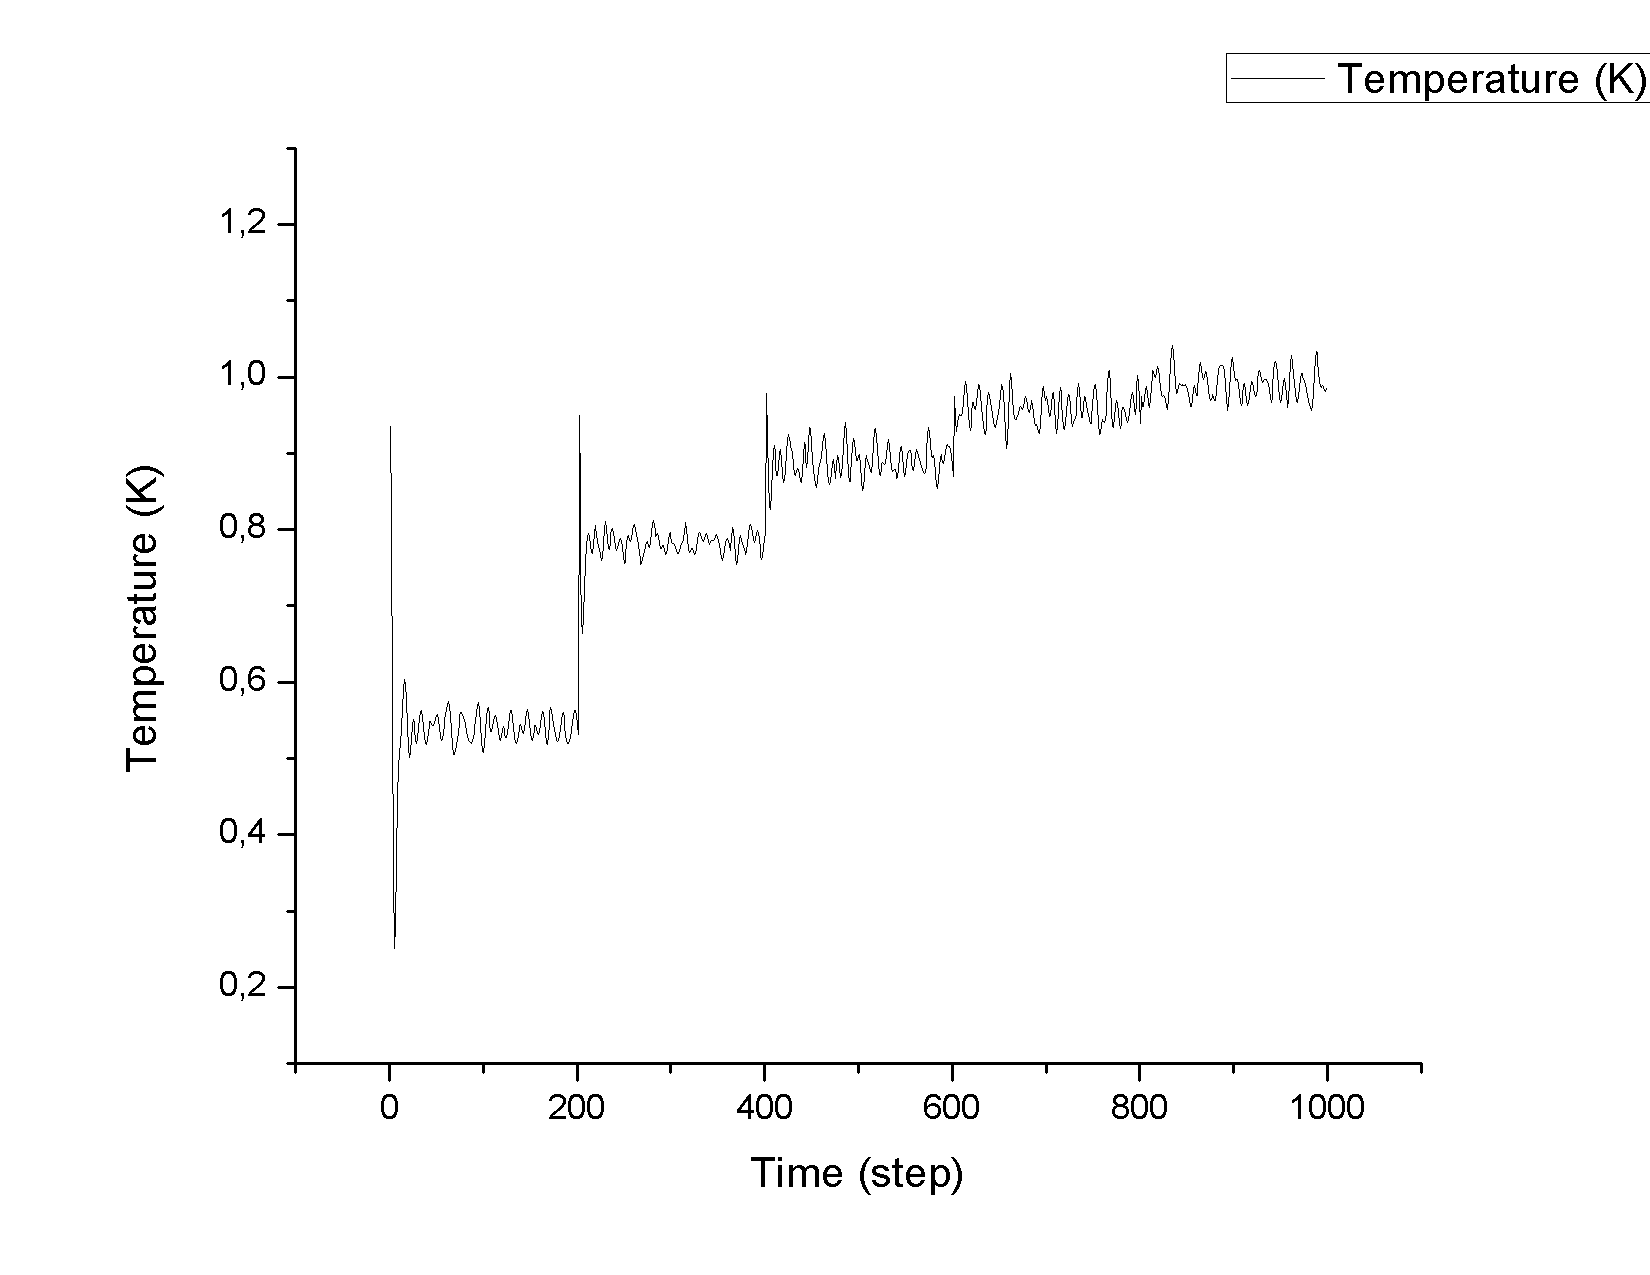
\includegraphics[width=0.75\textwidth]{md3}
    \caption{md3.cpp kimenete }
\end{figure}

\subsection{3.Feladat }
A kódon végzet modosításokat a függelékben közlöm.


\begin{figure}[H]
    \centering
    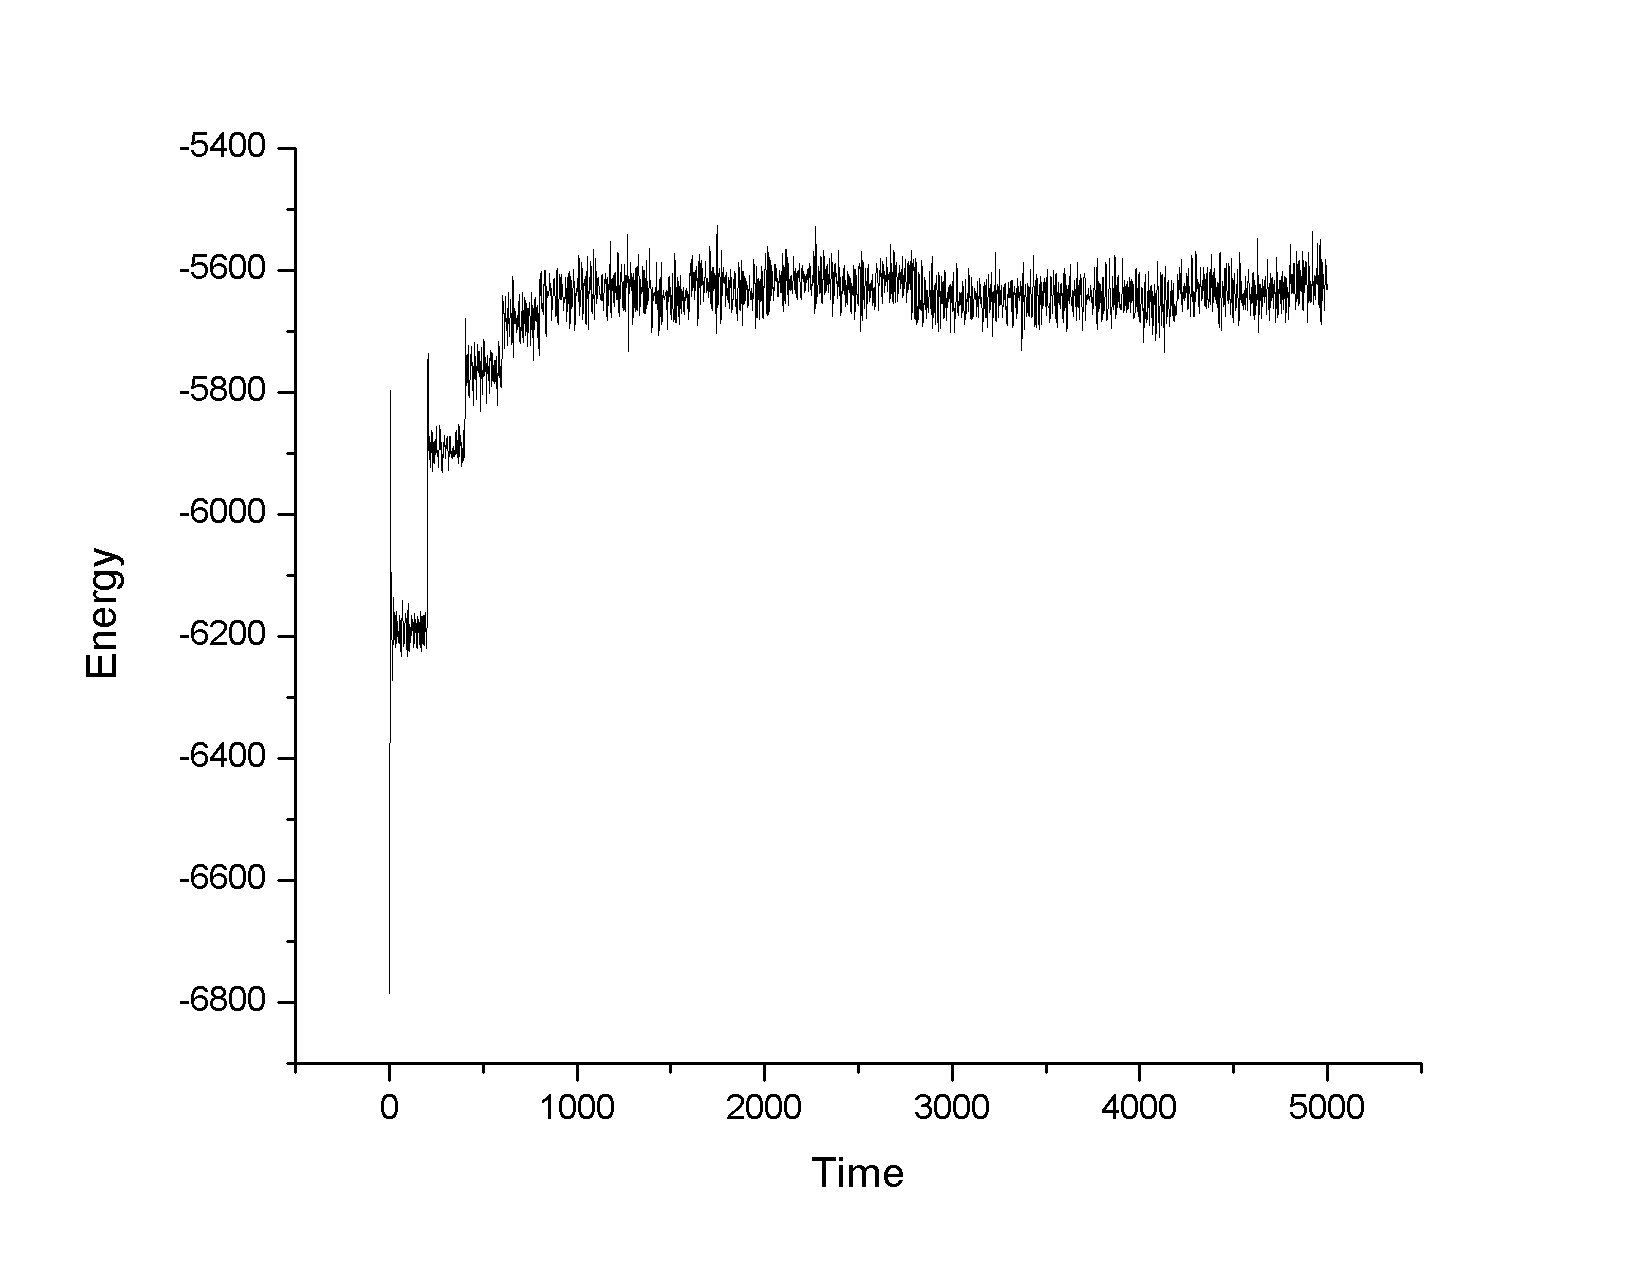
\includegraphics[width=0.75\textwidth]{E}
    \caption{energia}
\end{figure}


\begin{figure}[H]
    \centering
    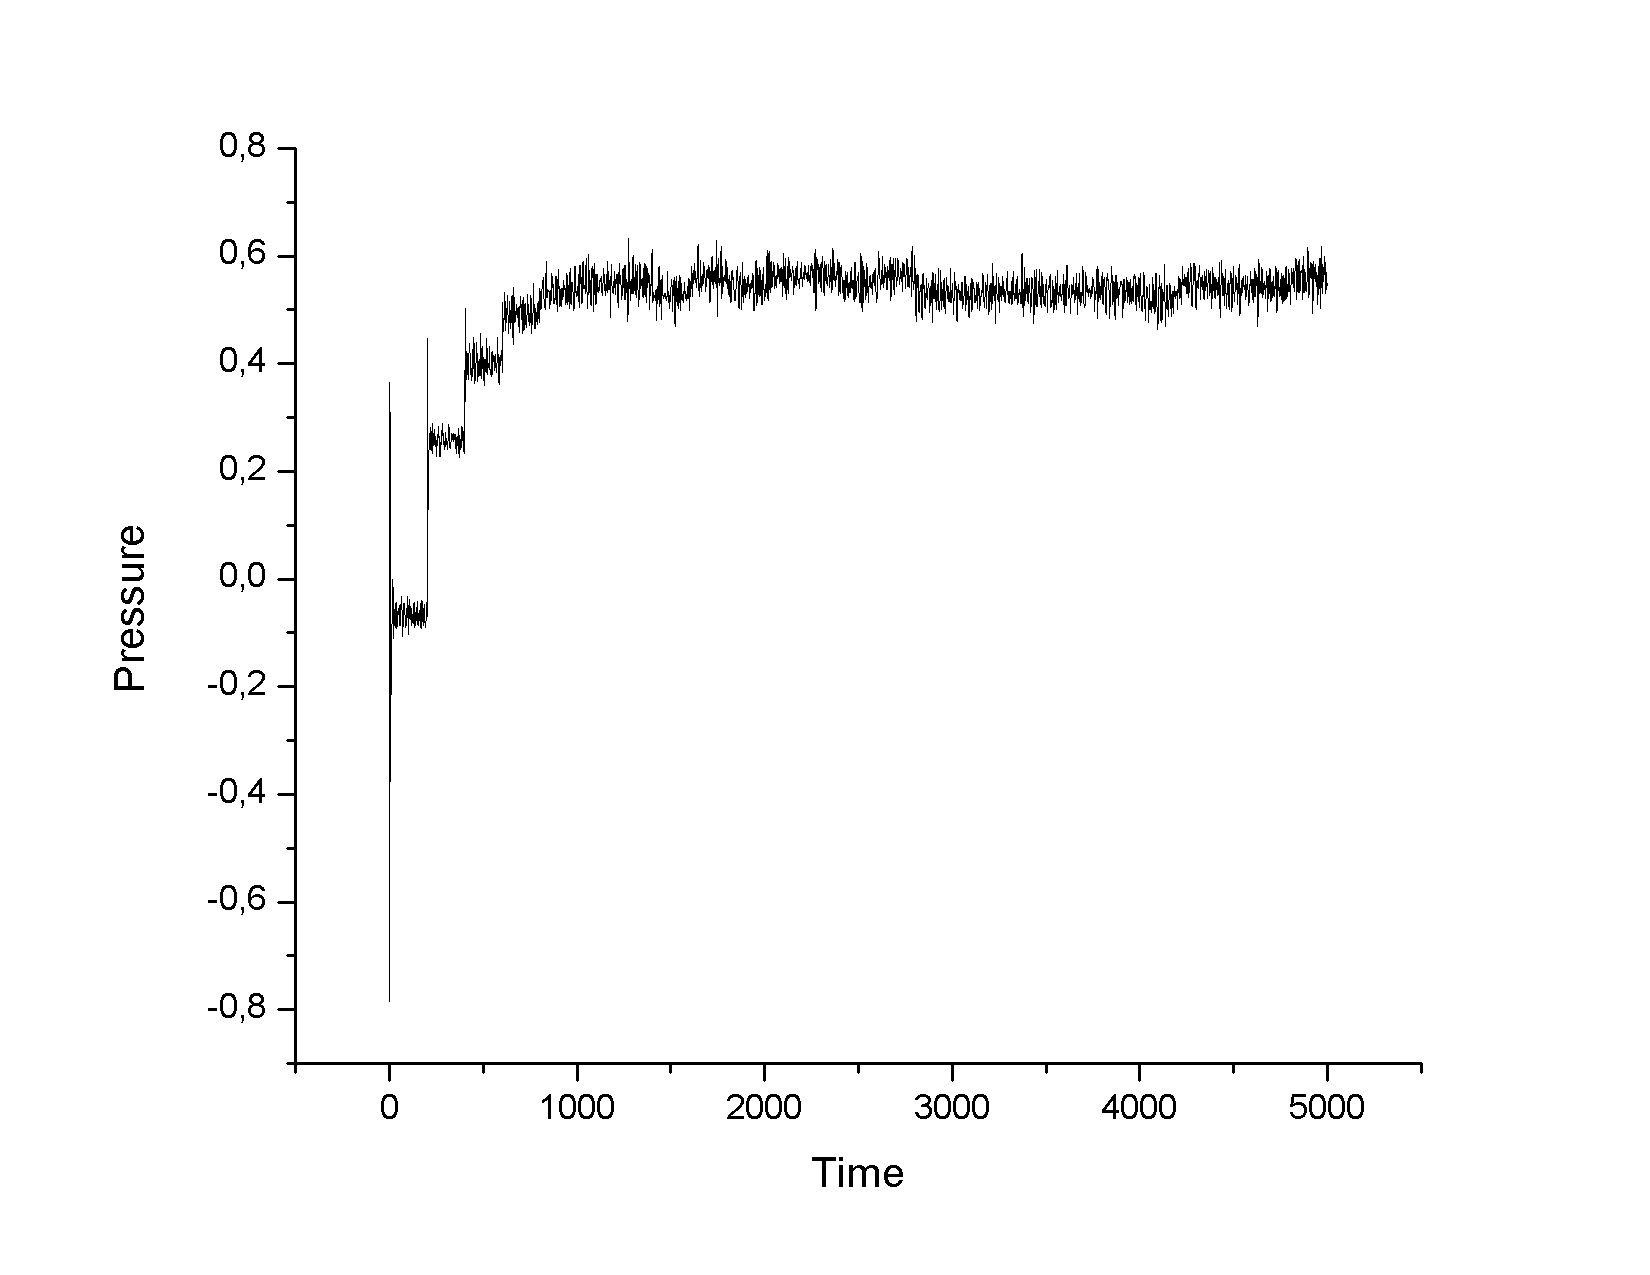
\includegraphics[width=0.75\textwidth]{P}
    \caption{nyomás}
\end{figure}

\begin{figure}[H]
    \centering
    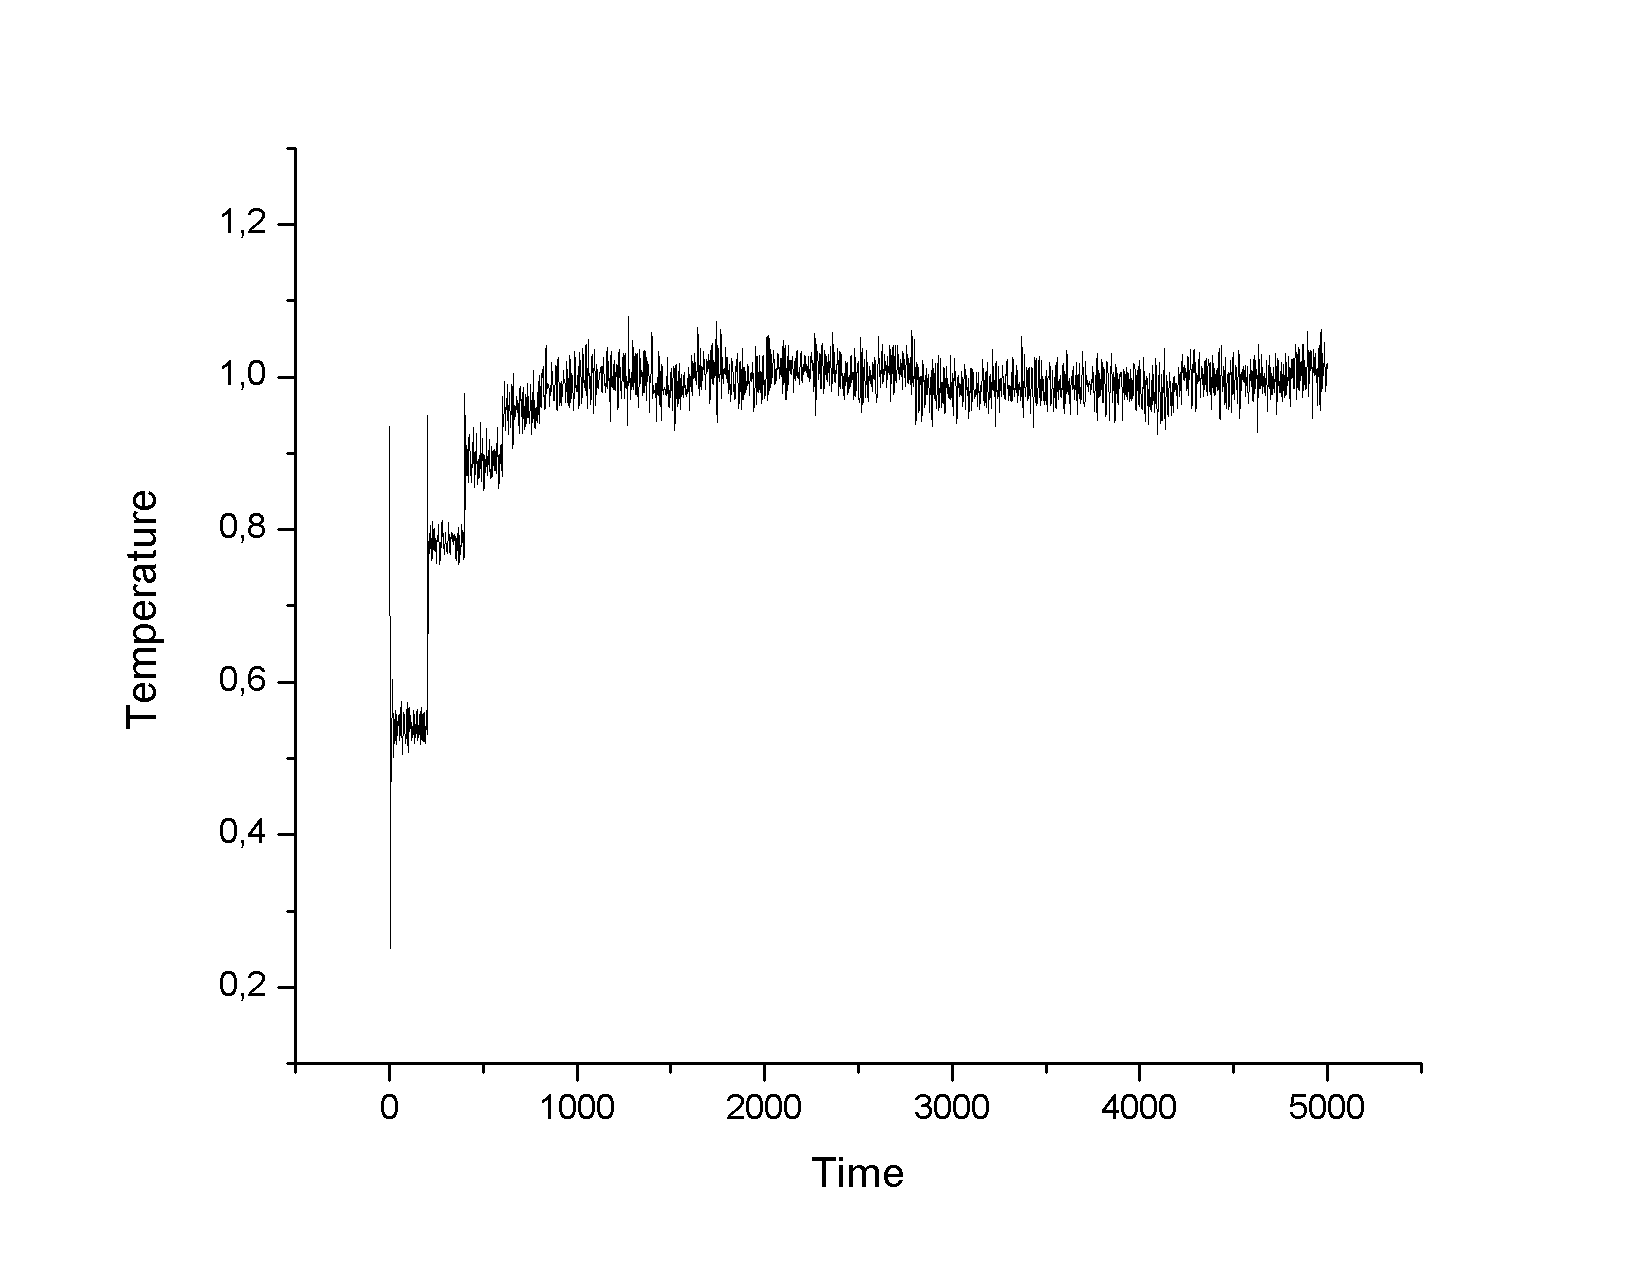
\includegraphics[width=0.75\textwidth]{T}
    \caption{hőmérséklet}
\end{figure}


\begin{figure}[H]
    \centering
    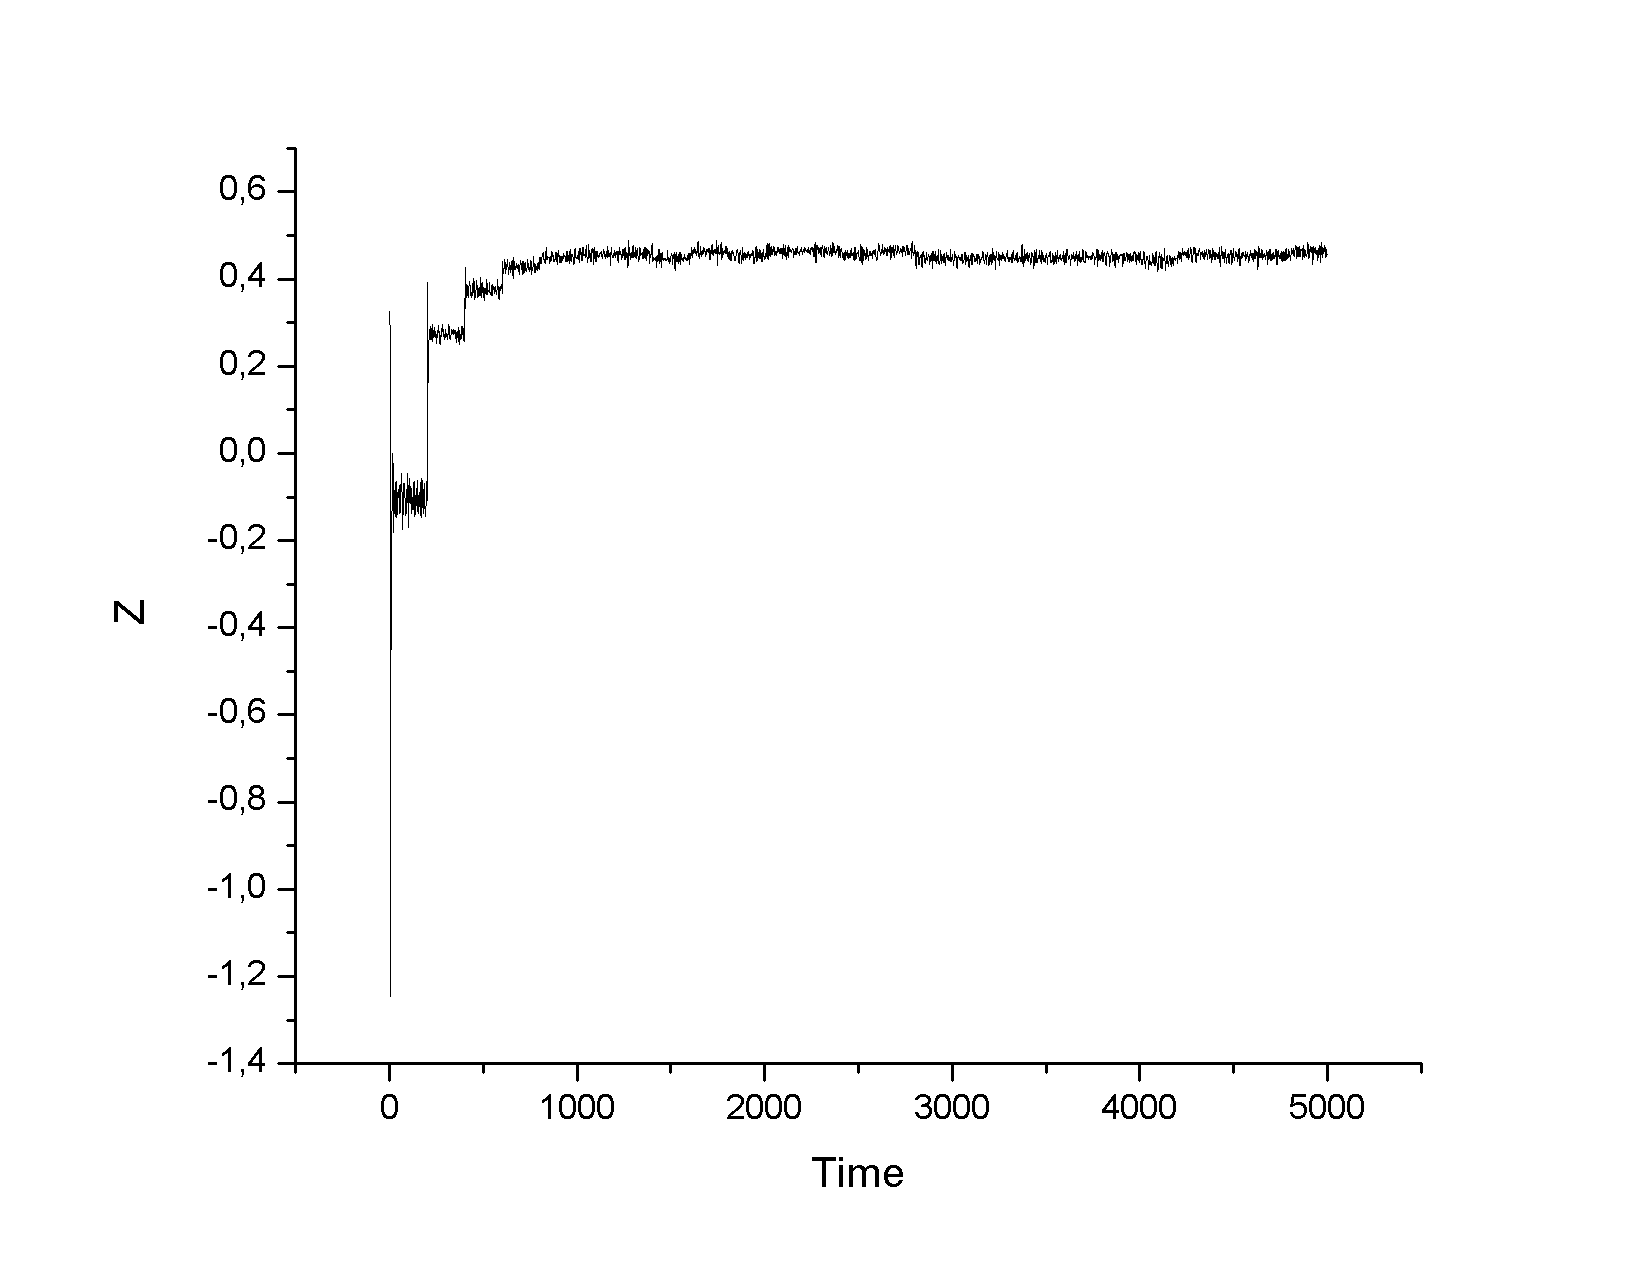
\includegraphics[width=0.75\textwidth]{Z}
    \caption{Kompresszibilítási tényező}
\end{figure}

\begin{figure}[H]
    \centering
    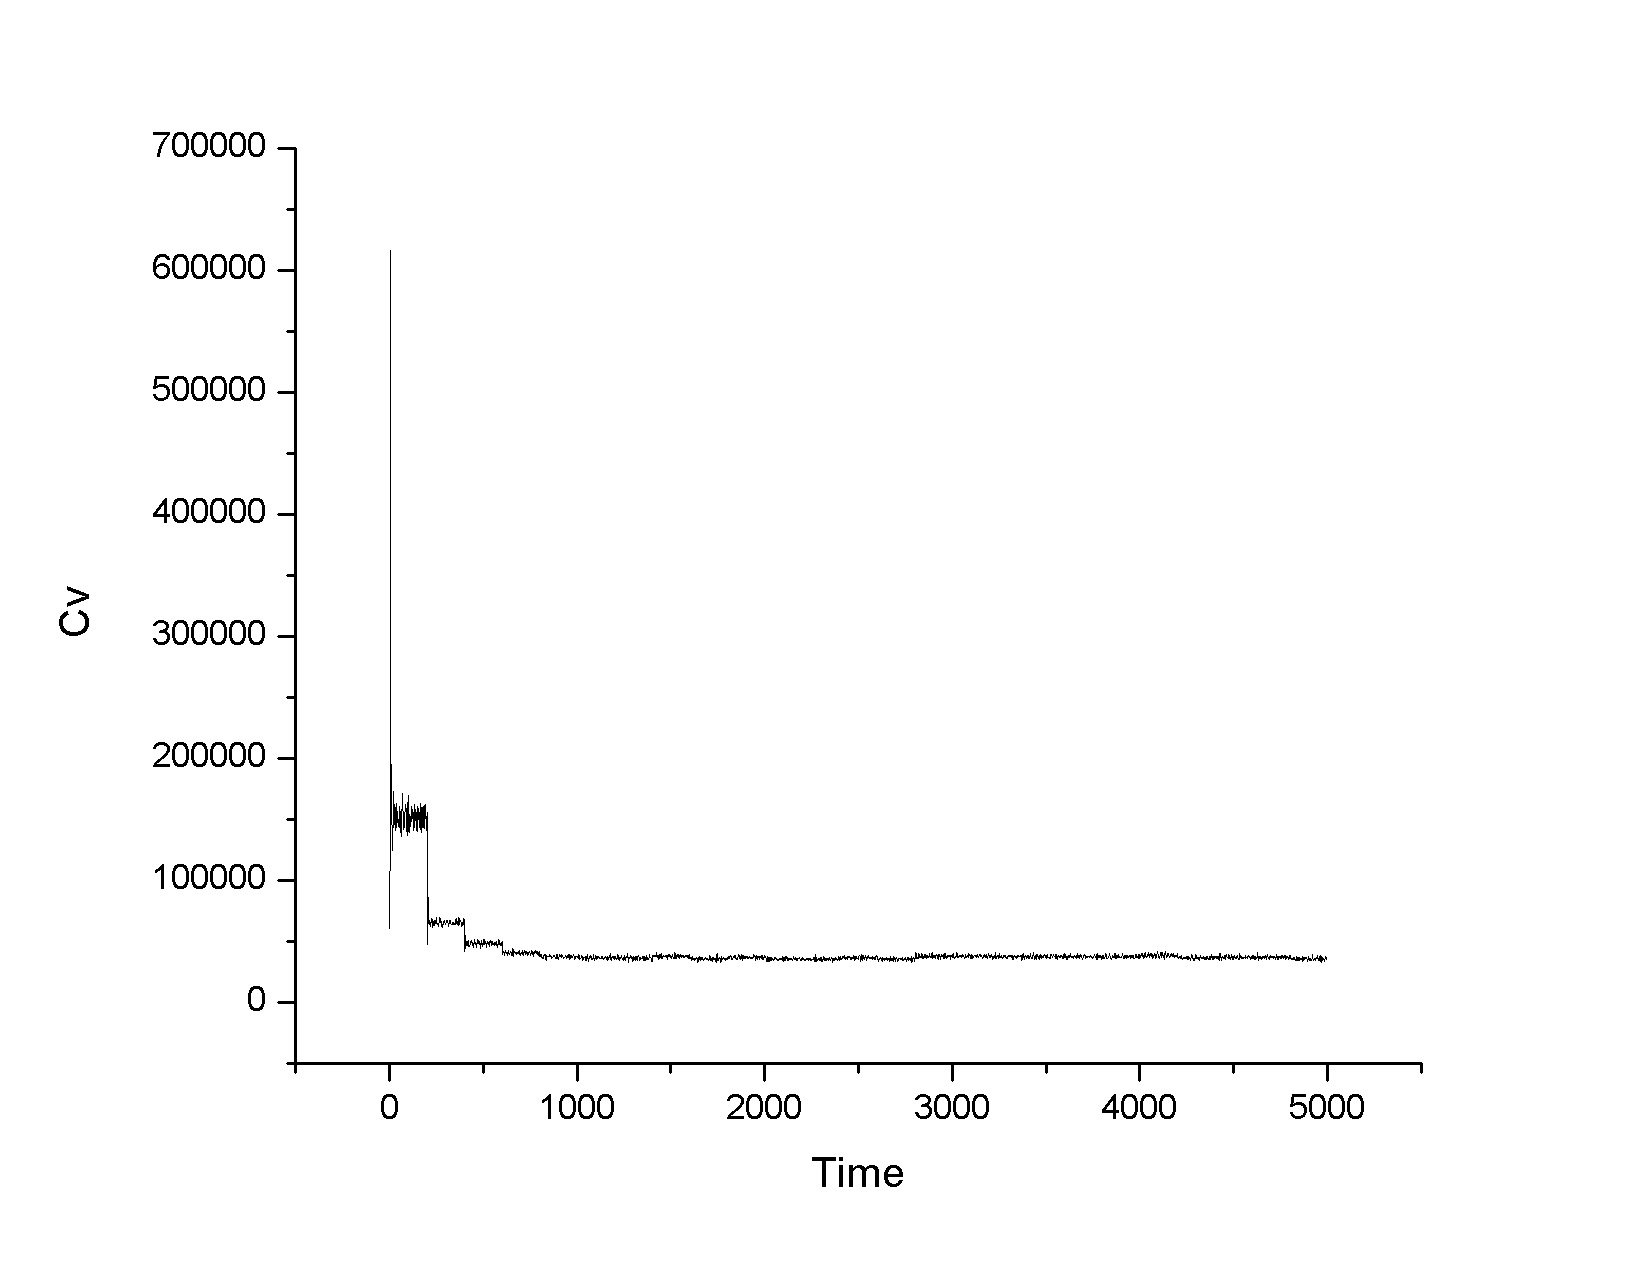
\includegraphics[width=0.75\textwidth]{cv}
    \caption{Fajhő}
\end{figure}



\newpage
\section{Függelék}
\subsection{A 3. feladathoz a modosított md3.cpp kód}
\begin{verbatim}
int main() {
    clock_t start = clock();
    initialize();
    updatePairList();
    updatePairSeparations();
    computeAccelerations();
    double dt = 0.01;
    ofstream file("T3.data");
//    file << "% Energy" << "\t" << "T" << "\t" << "P" << "\t" << "Z" << "\t" << "Cv" << endl;
    double a_sum = 0;
    double out_T = 0;
    double E = 0;
    double E_2 = 0;
    double Energy = 0;   
    double Ek=0;
    for (int i = 0; i < 5000; i++) {
        velocityVerlet(dt);
        a_sum = 0.;
        Ek = 0.;
        for(int j=0; j<N;j++){
            for(int k=0; k<3;k++){
                Ek=+pow(v[j][k],2);
            }       
        }
            for (int p = 0; p < nPairs; p++) {
            a_sum+=pow(1/rSqdPair[p],6)-pow(1/rSqdPair[p],3);
            }
        Energy=Ek/2+4*a_sum;
        file << i <<"\t" <<  Energy << "\t" << (out_T=instantaneousTemperature()) << "\t" <<
        (N*out_T+(1.0/3)*a_sum)/(pow(L,3)) << "\t" << (N*out_T+(1.0/3)*a_sum)/(N*out_T) << "\t";
        E_2 = pow(Energy, 2);
        E = Energy;
        file << (((E_2/N)-pow((E/N), 2))/(pow(out_T, 2))) << endl;
        if (i % 200 == 0)
            rescaleVelocities();
        if (i % updateInterval == 0) {
            updatePairList();
            updatePairSeparations();
        }
    }
    file.close();
    clock_t stop = clock();
double time = (double)(stop-start)/CLOCKS_PER_SEC;
ofstream proc("time.dat");
proc << "szamitasi ido: " << time;
proc.close();
}
\end{verbatim}




\begin{thebibliography}{2}
\bibitem{jegyzet} 
Jegyzet
\\\texttt{$https://stegerjozsef.web.elte.hu/teaching/szamszim/moldin.pdf$}
 
\bibitem{forraskod} 
Forráskód
\\\texttt{$https://stegerjozsef.web.elte.hu/teaching/szamszim/moldin.tgz$}

\end{thebibliography}













\end{document}

